\section{Deep Deterministic Policy Gradient (DDPG)}\label{DDPG}
As mentioned in \Cref{sec:DQN} the Deep Q-Network solves problems with high-dimensional observation space. But the problem is it can only handle discrete and low-dimensional action space. Many tasks of interest, most notably physical control tasks, have continuous (real-valued) and high-dimensional action spaces. The problem with the Deep Q-Network is it cannot be applied to continuous domains since it relies on finding the action that maximizes action-value function. In the continuous valued case requires an iterative optimization process at every step. \cite{DBLP:journals/corr/LillicrapHPHETS15}

An obvious approach to adapting the Deep Q-Network method to the continuous domain is to simply discretize the action space. This has many limitations, most important the curse of dimensionality - the number of actions increases exponentially with the number of degrees of freedom. An example is the human arm has 7 degrees of freedom, with an assumption discretization $a_i \sim  \{-k,0,k\}$ for each joint leads to an action space with dimensionality: $3^7 = 2187$. This problem just becomes bigger with a finer discretion. Such a large action space makes it difficult to explore efficiently. Discretization of action spaces throws away information of the action domain.

The Deep Deterministic Policy Gradient tries to solve these problems. The Deep Deterministic Policy Gradient method is a model-free off-policy actor-critic algorithm using deep function approximators that can learn policies in high-dimensional, continuous action space. 

The DDPG algorithm uses some of the same deep learning tricks as the Deep Q-Network (DQN) see \Cref{sec:DQN}. To explain more about this algorithm a car simulation environment called TORCS (The Open Racing Car Simulator) is used - see \Cref{sec:TORCS} for more information about the TORCS environment \cite{DDPG_Torcs}.


\subsection{Algorithm}
Even with the DDPG using some of the tricks from the DQN algorithm, it is not straightforward to apply the Q-learning to continuous action space. It is because of the continuous action space finding a greedy policy requires an optimization of \textit{$a_t$} at every time step - this optimization is too slow to be practical with large, unconstrained function approximators and non-trivial action spaces. Here is instead used an actor-critic approach based on the DPG (deterministic policy gradient) algorithm \cite{DBLP:conf/icml/SilverLHDWR14} 

The DPG algorithm uses a parameterized actor function $\mu(s|\theta^\mu)$ which specifies the current policy by deterministically mapping states to a specific action. The critic $Q(s,a)$ is learned by using the Bellman equation as in Q-learning. The actor is updated by applying the chain rule to the expected return from the start distribution J with respect to the actor parameters: 
 
\begin{equation}
\triangledown_{\theta^\mu} J \approx \mathbb{E}_{s_t \sim \rho^\beta} [\triangledown_{\theta^\mu}Q(s,a|\theta^Q)|_{s=s_t , a=\mu(s_t|\theta^\mu)}]  
\newline
\end{equation}
\begin{equation}
\triangledown_{\theta^\mu} J = \mathbb{E}_{s_t \sim \rho^\beta} [\triangledown_{a}Q(s,a|\theta^Q)|_{s=s_t , a=\mu(s_t)} \triangledown_{\theta_\mu}\mu(s|\theta^\mu)|_{s=s_t} ]
\end{equation} 

This was proved that it is the policy gradient - the gradient of the policy performance. 

Introducing nonlinear function approximators means that convergence is no longer guaranteed. The approximators are essential to learn and generalize on large state spaces. The DDPG contribution is to provide a modification to DPG inspired of the success of the DQN, which allow it to use neural networks function approximators to learn in state and action space online.  

One of the challenges of using neural networks for reinforcement learning is most optimization algorithms assume that the samples are independently and identically distributed. To solve this problem a replay buffer is used, it samples a minibatch uniformly from the buffer - more about the replay buffer see \Cref{sec:DQN}. Because the DDPG is an off-policy algorithm, the replay buffer can be large, allowing the algorithm to benefit from learning a set of uncorrelated transition.


\subsubsection{Update weights}
Directly implementing the Q-learning with neural networks is unstable in many environments. Since network $Q(s,a|\theta^Q)$ being updated is also used in calculating the target value, the Q-update is likely to divergence. It is modified from the DQN algorithm for actor-critic using "soft" target updates, instead of directly updating the weights. This is done by creating a copy of the actor and critic networks, $Q'(s,a|\theta^{Q'})$ and $\mu'(s|\theta^{\mu'})$ respectively, they are used for calculating the target values. The weights of these target networks are then updated by having them slowly track the learned networks: 
\begin{equation}
\theta' \leftarrow \tau \theta + (1-\tau)\theta'   \quad \textrm{with} \quad \tau \ll 1 
\end{equation}   
This means that the target values are constrained to change slowly, greatly improving the stability of learning. This change helps the unstable problem of learning the action-value function closer to the case of supervised learning, where a robust solution exists. The DDPG needs both a target $\mu'$ and $Q'$ was required to have stable targets $y_i$ to consistently train the critic without divergence. It may slow learning since the target network delays the propagation of value estimations. In practice, it is better because the stability of training is more important than the learning speed.

\subsubsection{Batch normalization}
Different components of the observation may have different physical units (for example, position versus velocities) and the ranges may change through the different environments. This can make it difficult for the network to learn effectively and may make it difficult to find hyper-parameters which generalize across environments with different scales of state values.

One approach to solving this problem is to manually scale the features so they have similar ranges across different environments and units. The way this problem is solved in the DDPG algorithm is by using a technique for deep learning called batch normalization. This technique normalizes each dimension across the samples in a minibatch to have a unit mean and variance. It maintains a running average of the mean and variance to use for normalization during training, in the DDPG for exploration or evaluation. In a low-dimensional case the batch normalization is used on the state input and all layers of the actor network ($\mu$-network) and all layers of the critic network ($Q$-network) prior to the action input. With batch normalization, the DDPG is able to learn effectively across many different tasks with different types of units, without needing to manually ensure units in different ranges.

\subsubsection{Exploration}
A major challenge of learning continuous action spaces is exploration. An advantage of an off-policy algorithm such as DDPG is that it can treat problems of exploration independently from learning algorithm. The DDPG has an exploration policy $\mu'$ by adding noise sampled from a noise process $N$ to the actor policy: 
\begin{equation}
\mu'(s_t) = \mu(s_t|\theta_t^\mu) + N
\end{equation} 
N can be chosen to suit the environment. The noise can be added using a process called Ornstein-Uhlenbeck to do the exploration.

The DDPG algorithm can be seen on \Cref{algo:DDPG}, it is the algorithm DeepMind uses \cite{DBLP:journals/corr/LillicrapHPHETS15}.  



\begin{algorithm}[H]
	\caption{Deep Deterministic Policy Gradient (DDPG) algorithm}
	\label{algo:DDPG}
	\begin{algorithmic}[H]
		\State Randomly Initialize critic network $Q(s,a|\theta^Q)$ and actor $\mu(s|\theta^\mu)$ with weights $\theta^Q$ and $\theta^\mu$
		\State Initialize target network $Q'$ and $\mu'$ with weights $\theta^{Q'} \leftarrow \theta^{Q}, \theta^{\mu'} \leftarrow \theta^{\mu}$ 
		\State Initialize replay Buffer $R$
		\For {$episode = 1$ to M} 
			\State Initialize a random process $N$ for action exploration
			\State Receive initial observation state $s_1$
			\For {$t = 1$ to T}
				\State Select action $a_t = \mu(s_t|\theta^\mu + N_t)$ according to the current policy and exploration noise
				\State Store transition $(s_t,a_t,r_t,s_{t+1})$ in $R$
				\State Sample random minibatch of $N$ transitions$(s_i,a_i,r_i,s_{i+1})$ from $R$
				\State Set $y_i = r_i+\gamma Q'(s_{i+1},\mu'(s{i+1}|\theta^{\mu'})|\theta^{Q'})$
				\State Update critic by minimizing the loss: $L=\frac{1}{N} \sum_{i}(y_i - Q(s_i,a_i|\theta^Q))^2$
				\State Update the actor policy using the sampled policy gradient:   
		  			   \begin{equation*}
		  			   \triangledown_{\theta^\mu} J = \frac{1}{N} \sum_{i} \triangledown_{a}Q(s,a|\theta^Q)|_{s=s_i , a=\mu(s_i)} \triangledown_{\theta_\mu}\mu(s|\theta^\mu)|_{s=s_i} 
		  			   \end{equation*}
		  		\State Update the target networks:
		  			   \begin{equation*}
		  			   \theta^{Q'} \leftarrow \tau \theta^Q + (1-\tau)\theta^{Q'} 
		  			   \end{equation*}
		  			   \begin{equation*}
		  			   \theta^{\mu'} \leftarrow \tau \theta^\mu + (1-\tau)\theta^{\mu'} 
		  			   \end{equation*}
			\EndFor
		\EndFor
	\end{algorithmic}
\end{algorithm}


\subsection{Network}
To use the DDPG algorithm 3 networks need to be created, an actor network, a critic network, and a target network. To understand the structure of these networks, we will use an example from the TORCS environment \cite{DDPG_Torcs}. In this example, the input is the sensor data from the car used as the state of the environment. It has 29 different sensor inputs \cite{Data_from_Torcs}, so the state space has the size of 29.  

Before the actor and critic network are explained, the actor-critic algorithm will be explained. The actor-critic algorithm is a hybrid method which combines the policy gradient method and the value function method. The policy is known as the actor, while the value function is the critic. The actor produces an action $a$ given the current state of the environment $s$. The critic then produces a signal to criticizes the actions made by the actor. To refer to the human world is this a normal behavior, where the junior employee (actor) do the actual job and his boss (critic) criticizes the work and hopefully the junior employee can do it better next time. In the TORCS example, it uses the continuous Q-learning (SARSA) as the critic model and uses policy gradient method as the actor model. The following figure explains the relationships between Value Function, Policy Function, and actor-critic algorithm.    

The tricks from the Deep Q-Network is used, where the Q-function is replaced with a neural network $Q^\pi(s,a) \approx Q(s,a,w)$ where w is the weight of the neural network. This ends up with the formula for Deep Deterministic Policy Gradient:
 
\begin{equation}
\frac{\partial L(\theta)}{\partial \theta} =\frac{\partial Q(s,a,w)}{\partial a} \frac{\partial a}{\partial \theta}
\end{equation}
Where the policy parameters $\theta$ can be updated via stochastic gradient ascent.

As in the DQN, an iterative method is used to solve the Q-function, where the loss function is:
\begin{equation}
Loss = [r + \gamma Q(s',a') - Q(s,a)]^2
\end{equation} 

The Q-value can be used to estimate the values of the current actor policy. The actor-critic algorithm can be seen on figure \Cref{fig:Actor_critic_architecture}. 

\begin{figure}[H]
	\centering
	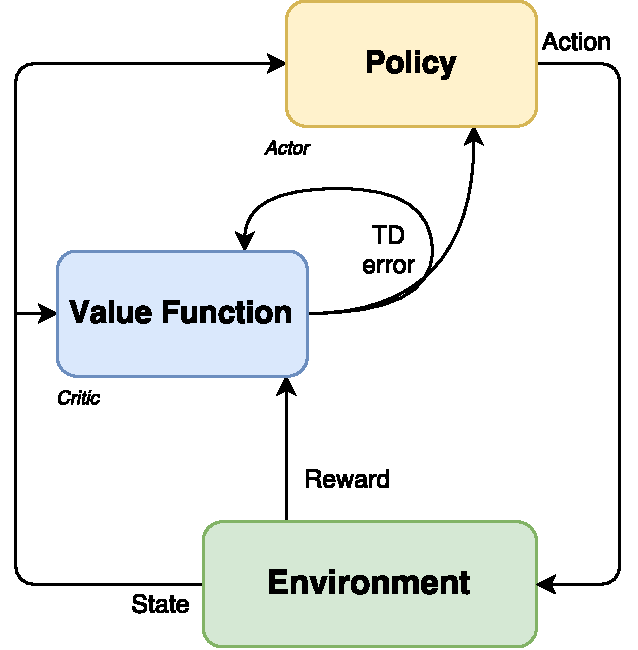
\includegraphics[width=0.6\textwidth]{Figures/Architecture/DDPG/Actor_critic_architecture.pdf}
	\caption{Actor-critic algorithm which is used in DDPG}
	\label{fig:Actor_critic_architecture}
\end{figure}

\subsubsection{Actor network}
The actor-network is created using two hidden layers with 300 hidden units and 600 hidden units. The output consists of three continuous actions, Steering, which is a single unit with tanh activation function (where -1 means turn maximum right and +1 means turn maximum left). Acceleration, which is a single unit with sigmoid activation function (where 0 means no gas, 1 means full gas). Brake, another single unit with sigmoid activation function (where 0 means no brake, 1 full brake). The actor network can be seen on \Cref{fig:DDPG_Actor_network}. The hidden layers are all fully connected layers. To be able to send the actions to the game the three different actions (steering, acceleration, and brake) must be merged to the same action.

\begin{figure}[H]
	\centering
	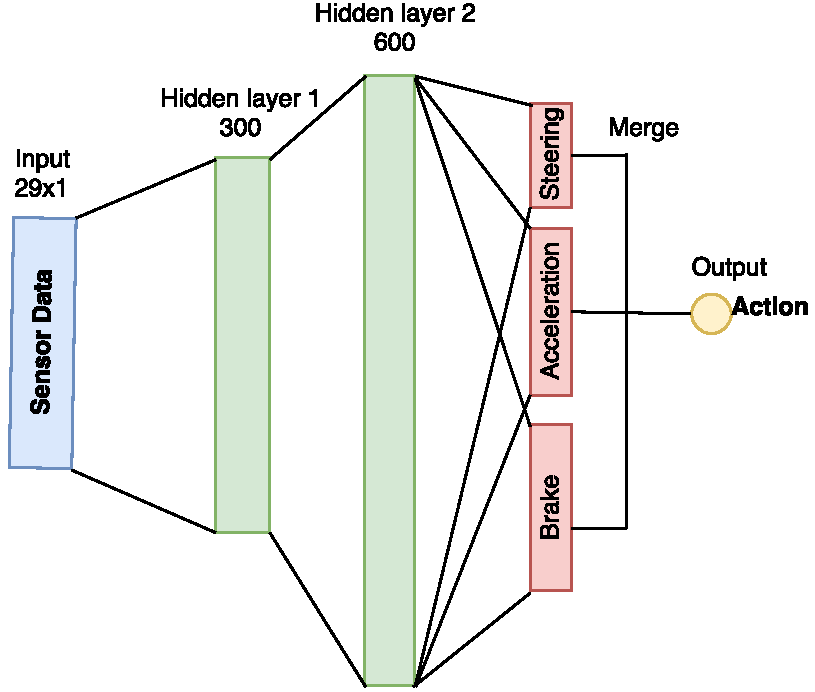
\includegraphics[width=0.7\textwidth]{Figures/Architecture/DDPG/DDPG_Actor_network.pdf}
	\caption{Actor network used in DDPG for playing TORCS }
	\label{fig:DDPG_Actor_network}
\end{figure}  


\subsubsection{Critic network}
The construction of the Critic Network is very similar to the Deep Q-Network described in \Cref{sec:DQN}. The only difference is that uses two hidden layers with 300 and 600 hidden units. The critic network takes both the states and the action as inputs. According to the DDPG paper \cite{DBLP:journals/corr/LillicrapHPHETS15}, the actions were not included in the 2’nd hidden layer of Q-network. This critic network can be seen on \Cref{fig:DDPG_Critic_network}. Of the figure is a third hidden layer shown, but it is still the second layer, just the state, merged with the actions in the original second layer. 

\begin{figure}[H]
	\centering
	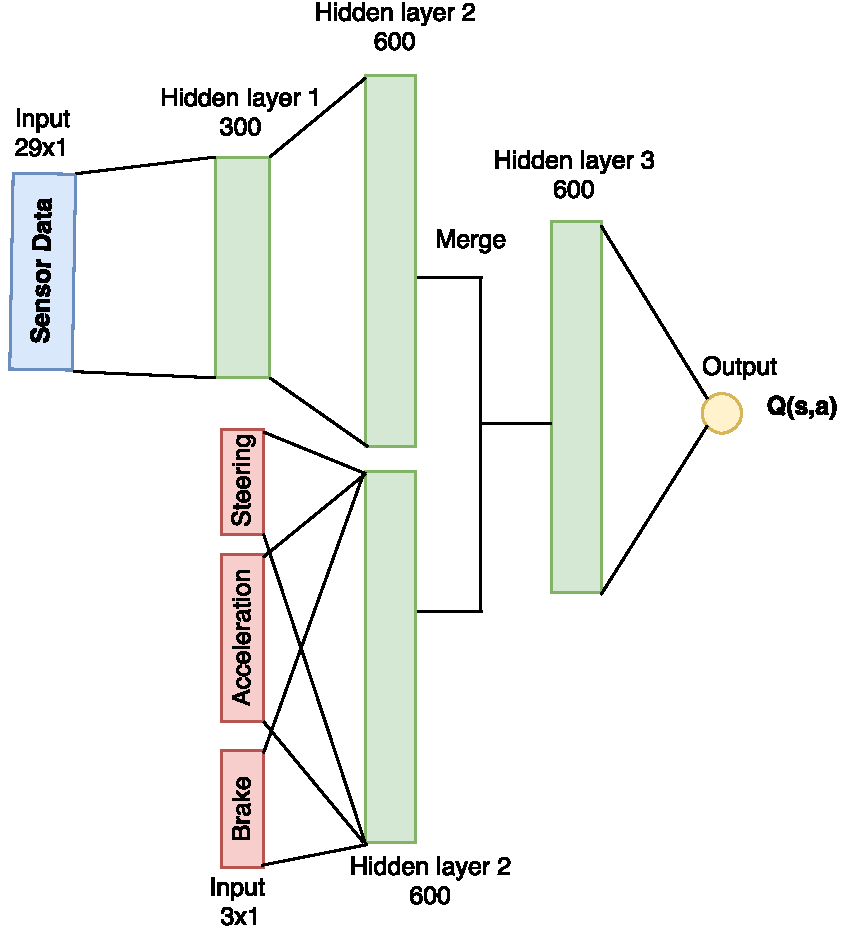
\includegraphics[width=0.7\textwidth]{Figures/Architecture/DDPG/DDPG_Critic_network.pdf}
	\caption{Critic network used in DDPG for playing TORCS }
	\label{fig:DDPG_Critic_network}
\end{figure}  

\subsubsection{Training}
The way the actor and critic network is used for learning how to play TORCS is: 
\begin{enumerate}
	\item The sensor data is received from the environment (TORCS) 
	\item The sensor input will be fed into the neural network, and the network will output 3 real numbers (value of the steering, acceleration, and brake)
	\item The network will be trained many times, via the Deep Deterministic Policy Gradient, to maximize the future expected reward.
\end{enumerate}

The actual training is not that complicated. First update the critic by minimizing the loss:
\begin{equation}
L = \frac{1}{N} \sum_{i} (y_i - Q(s_i,a_i|\theta^Q))^2
\end{equation}
\newpage
Then the actor policy is updated using the sampled policy gradient:
\begin{equation}
\triangledown_\theta J = \frac{\partial Q^\theta(s,a)}{\partial a} \frac{\partial a }{\partial \theta}
\end{equation}

$a$ is the deterministic policy: $a=\mu(s|\theta)$. It can be written as:
\begin{equation}
\triangledown_\theta J = \frac{\partial Q^\theta(s,a)}{\partial a} \frac{\partial \mu(a|\theta) }{\partial \theta}
\end{equation}

The last thing is to update the target network:
\begin{equation}
\theta^{Q'} \leftarrow \tau \theta^Q + (1-\tau)\theta^{Q'} 
\end{equation}
\begin{equation}
\theta^{\mu'} \leftarrow \tau \theta^\mu + (1-\tau)\theta^{\mu'} 
\end{equation}

The results of the DDPG in TORCS" can be found in Ben Lau blog "Using Keras and Deep Deterministic Policy Gradient to play TORCS" \cite{DDPG_Torcs}.